\section{Module 9. Segmentation}

Brain MRI segmentation is an essential task in many clinical applications
because it influences the entire analysis. This is because different
processing steps rely on accurate segmentation of anatomical regions.
For example, MRI segmentation is commonly used for measuring and visualizing
different brain structures, for delineating lesions, for analysing
brain development, and for image-guided interventions and surgical
planning.

\textit{MRI Processing} To prepare brain MRI for segmentation, it
is necessary to perform several preprocessing steps. (Fig. \ref{fig:Preprocessing}).

\begin{figure}[H]
\centering{}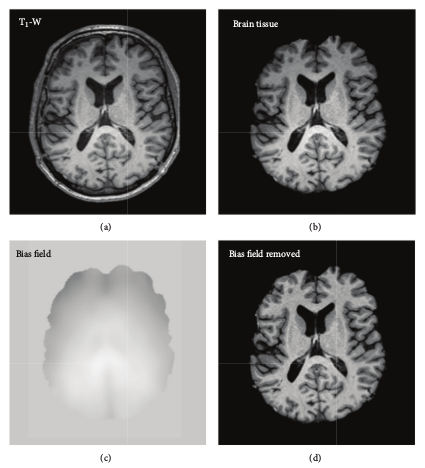
\includegraphics[scale=0.7,bb = 0 0 200 100, draft, type=eps]{9Preprocessing}\caption{Triangulation for the 15 patterns. \label{fig:Preprocessing}}
\end{figure}

The most important steps are: MRI bias field correction, image registration
and brain extraction.

\textit{Basic} An image for segmentation can be defined in 2D space
(pixels) or in 3D space (voxels). Each image element is specified
by its intensity value and coordinates for pixels (i,j) and for voxels
(i,j,k). Intensity values are typically represented by a gray value
{0, …, 255}.

The goal of image segmentation is to divide an image into a set of
semantically meaningful, homogeneous, and nonoverlapping regions of
similar attributes such as intensity, depth, color, or texture. Thesegmentation
result is either an image of labels identifying each homogeneous region
or a set of contours which describe the region boundaries.

Fundamental components of structural brain MRI analysis include the
classification of MRI data into specific tissue types and the identification
and description of specific anatomical structures. The problems of
segmentation and classification are interlinked because segmentation
implies a classification, while a classifier implicitly segments an
image. In the case of brain MRI, image elements are typically classified
into three main tissue types: white matter (WM), gray matter (GM),
and cerebrospinal fluid (CSF) (Fig. \ref{fig:Segment}).

\begin{figure}[H]
\centering{}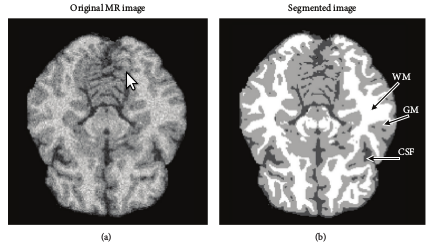
\includegraphics[scale=0.7,bb = 0 0 200 100, draft, type=eps]{9Segmentation}\caption{Triangulation for the 15 patterns. \label{fig:Segment}}
\end{figure}

One of the most important features for brain MRI segmentation is the
intensity of brain tissue. However, intensity-based segmentation algorithms
will lead to wrong results when intensity value are corrupted by MRI
artifacts.

\textit{MRI Segmentation Methods} There is no single method that can
be suitable for all images, nor are all methods equally good for a
particular type of image. For example, some of the methods use only
the gray level histogram, while some integrate spatial image information
to be robust for noisy environments. Some methods use probabilistic
or fuzzy set theoretic approaches, while some additionally integrate
prior knowledge (specific image formation model, e.g., MRI brain atlas)
to further improve segmentation performance. The segmentation methods,
with application to brain MRI, may be grouped as follows: 
\begin{itemize}
\item manual segmentation; 
\item intensity-based methods (including thresholding, region growing, classification,
and clustering); 
\item atlas-based methods; 
\item surface-based methods (including active contours and surfaces, and
multiphase active contours); 
\item hybrid segmentation methods. 
\end{itemize}
\hfill{}\\
\textbf{List of References}\\
\cite{09a1}